
\section{Methods and materials}

%To solve a problem like this there is generally two types of approaches, a theoretic approach where the models are derieved using physics and electromagnetism and an experimental approach where the PL is measured and a model is fitted to the data. %This article will focus on validation of existing models using experiments. 

This article has two parts to it the first is validation of PL models the second is to develop an extended PL model. The validation will be made over multiple steps, the first is to assume no knowledge of existing models and design a measurement campaign. The link of the measurement campaign can be seen in \autoref{link}. 

\begin{table}[!htbp]
\centering
\begin{tabular}{|c|c|}\hline
\textbf{Tx link}&\textbf{Rx link}\\\hline
Marconi instruments low noise & \multirow{2}{*}{Rx antenna} \\
signal generator 2042 (AAUNR. 33376) \\\hline
1.5 m SUCOFLEX\_104 & 2.5 m SUCOFLEX\_104 \\\hline 
\multirow{3}{*}{SMA male/male} & Rhode \& Schwarz FSL \\
&spectrum analyser \\
& (AAUNR. 56915)\\\hline
1 m RG223/U & \\\hline
Tx antenna &\\\hline
\end{tabular}
\caption{Equipment used for the Tx and Rx links in the measurement campaign.}
\label{link}
\end{table}
The measurement campaign accounts for six different parameters. 1) Two different locations, outside an empty parking lot as seen on \autoref{fig:test1} and inside a gym (45 by 25 meters) as seen on \autoref{fig:test2}. 2) Both horizontal and vertical polarization are tested. 3) Two different antenna structures have been tested, a set of monopole antennas (858 MHz) a set of patch antennas (858 MHz). 4) and 5) The height of the Tx and Rx antennas are varied\footnote{It is assumed that the PL for mirrored heights for example Rx = 0.04 m, Tx = 2.02 m and Rx at 2.02 m, Tx at 0.04 m is identical} between 0.04 m, 0.14 m, 0.36 m and 2.02 m. This is achieved by mounting the antennas on 2.5 m wooden poles using clamps. 6) The distance between Rx poles and Tx poles is varied across 1 m, 2 m, 4 m, 8 m, 15 m and 30 m. This gives 480 measurement points at each point 10 measurements are performed.

%A experiential method based on measurements is used to make the PL model, that will be used to calculate the loss for near ground communication. This model is based on data gathered from measuring the PL at different heights and distances. In each point there will be taken multiple measurements, so the noise factor will have a less of an effect on the results.

%During testing, five sets of antennas are used, a set monopole antennas (858 MHz) a set patch antennas (858 MHz). By using two different sets of antennas, it can be taken into account if the antenna type will have a influence on the results of the measurements. 

%There will also be tested with horizontal and vertical polarization, to see if this will effect the model. The testing will take place at two locations, outside an empty parking lot and inside a gym (45 by 25 meters). Two locations is used, to see if the model works at two different locations.








%\begin{figure}[!htbp]
%\centering
%
\includegraphics[width=0.2\textwidth]{Pplads.jpg}
%\caption{Illustration of the First and Second Fresnel zone, along with the Direct signal travelling from the Transmitter TX to the Receiver RX}
%\label{dijdk}
%\end{figure}

%\captionsetup{belowskip=-6.5em}
\begin{figure}[H]
\centering
\begin{minipage}{.23\textwidth}
  \centering
  
\includegraphics[width=\linewidth]{Pplads.jpg}
  \captionof{figure}{Measurement at the empty parking lot}
  \label{fig:test1}
\end{minipage}%
\hspace{2mm}
\begin{minipage}{.23\textwidth}
  \centering
  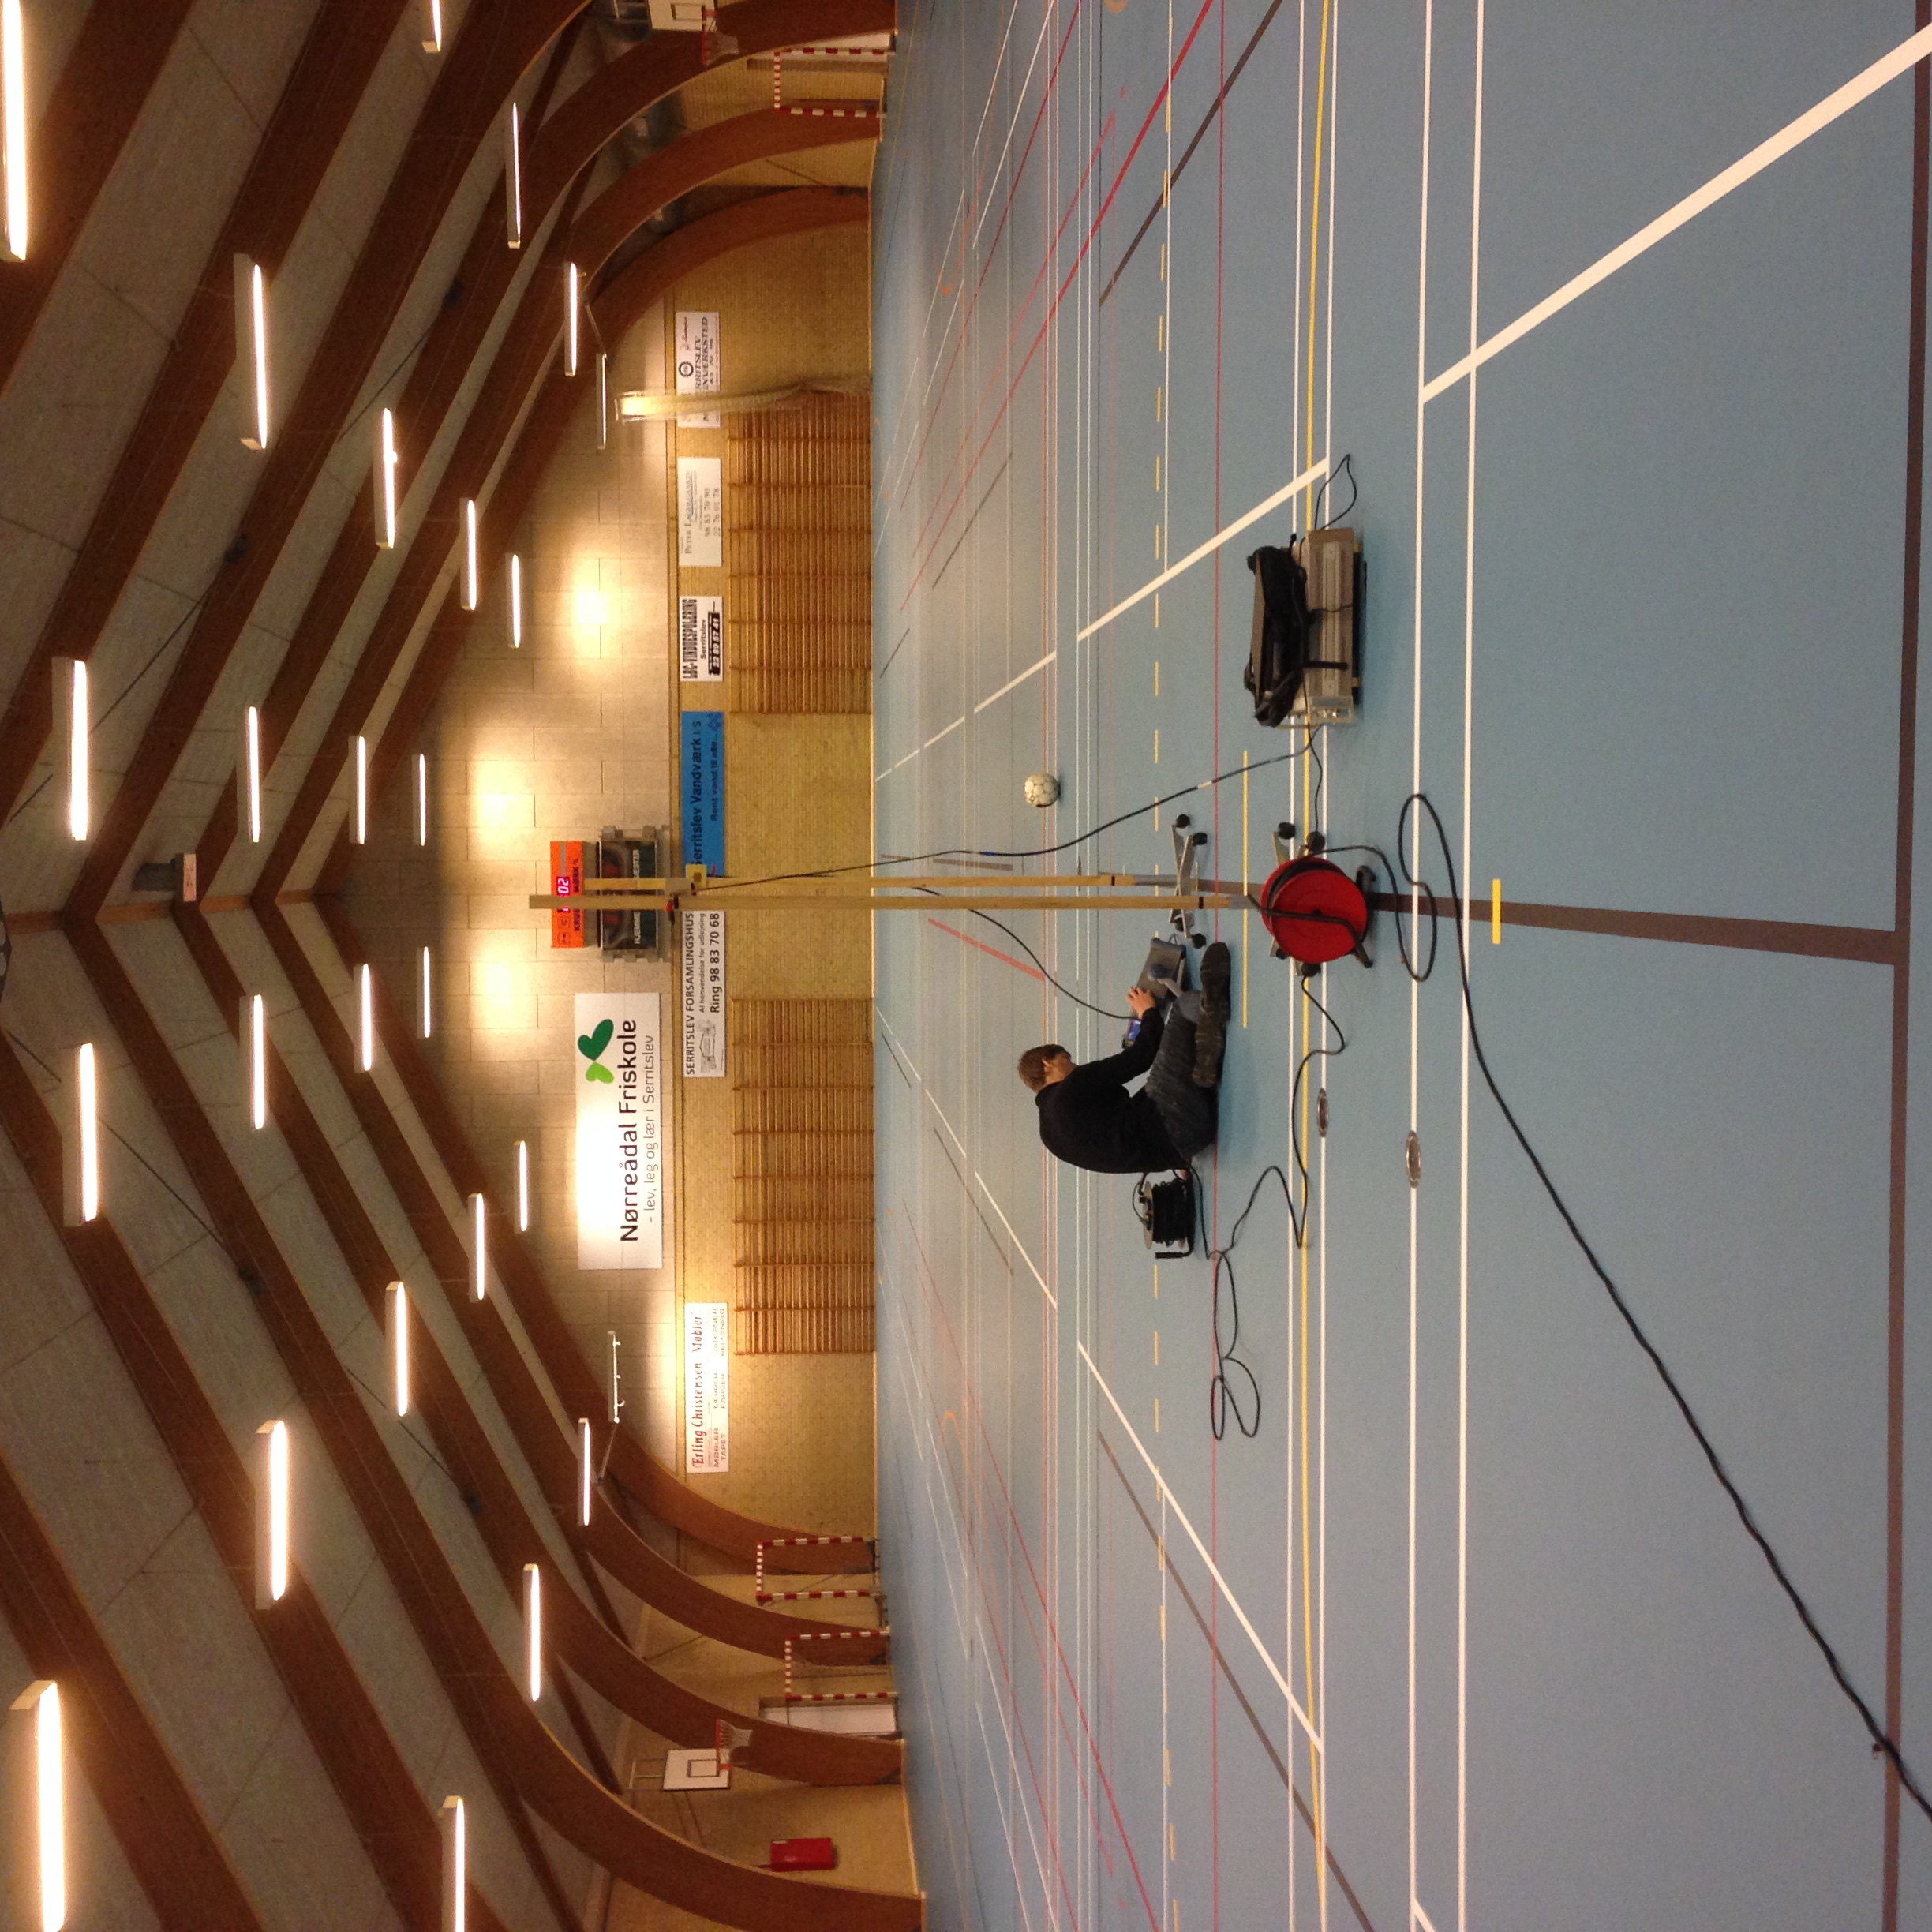
\includegraphics[angle=-90, width=\linewidth]{Hal.jpg}
  \captionof{figure}{Measurement at the gym}
  \label{fig:test2}
\end{minipage}
\end{figure}

To minimize uncertainties at the individual test points a mean of 10 measurements is found. Next the received power is adjusted according to $P_t$, $G_t$, $G_r$ and $L$ to find the pure PL. The next step of the validation is to exclude parameters that have little to no statistical influence on the PL. Lastly the models will be used to predict the PL, which will be matched with the data to verify the accuracy of the predictions using the mean square error (MSE) method.  